\documentclass{extbook}[14pt]
\usepackage{multicol, enumerate, enumitem, hyperref, color, soul, setspace, parskip, fancyhdr, amssymb, amsthm, amsmath, latexsym, units, mathtools}
\everymath{\displaystyle}
\usepackage[headsep=0.5cm,headheight=0cm, left=1 in,right= 1 in,top= 1 in,bottom= 1 in]{geometry}
\usepackage{dashrule}  % Package to use the command below to create lines between items
\newcommand{\litem}[1]{\item #1

\rule{\textwidth}{0.4pt}}
\pagestyle{fancy}
\lhead{}
\chead{Answer Key for Progress Quiz 5 Version C}
\rhead{}
\lfoot{8497-6012}
\cfoot{}
\rfoot{Summer C 2021}
\begin{document}
\textbf{This key should allow you to understand why you choose the option you did (beyond just getting a question right or wrong). \href{https://xronos.clas.ufl.edu/mac1105spring2020/courseDescriptionAndMisc/Exams/LearningFromResults}{More instructions on how to use this key can be found here}.}

\textbf{If you have a suggestion to make the keys better, \href{https://forms.gle/CZkbZmPbC9XALEE88}{please fill out the short survey here}.}

\textit{Note: This key is auto-generated and may contain issues and/or errors. The keys are reviewed after each exam to ensure grading is done accurately. If there are issues (like duplicate options), they are noted in the offline gradebook. The keys are a work-in-progress to give students as many resources to improve as possible.}

\rule{\textwidth}{0.4pt}

\begin{enumerate}\litem{
Solve the rational equation below. Then, choose the interval(s) that the solution(s) belongs to.
\[ \frac{5}{7x + 6} + -7 = \frac{-6}{-28x -24} \]The solution is \( x = -0.786 \), which is option D.\begin{enumerate}[label=\Alph*.]
\item \( x_1 \in [-1.4, -0.7] \text{ and } x_2 \in [0.1,1.6] \)

$x = -0.786 \text{ and } x = 0.929$, which corresponds to getting the correct solution and believing there should be a second solution to the equation.
\item \( \text{All solutions lead to invalid or complex values in the equation.} \)

This corresponds to thinking $x = -0.786$ leads to dividing by zero in the original equation, which it does not.
\item \( x_1 \in [-1.4, -0.7] \text{ and } x_2 \in [-2,0.3] \)

$x = -0.786 \text{ and } x = -0.633$, which corresponds to getting the correct solution and believing there should be a second solution to the equation.
\item \( x \in [-1.79,1.21] \)

* $x = -0.786$, which is the correct option.
\item \( x \in [0.7,2] \)

$x = 0.929$, which corresponds to not distributing the factor $7x + 6$ correctly when trying to eliminate the fraction.
\end{enumerate}

\textbf{General Comment:} Distractors are different based on the number of solutions. Remember that after solving, we need to make sure our solution does not make the original equation divide by zero!
}
\litem{
Choose the equation of the function graphed below.

\begin{center}
    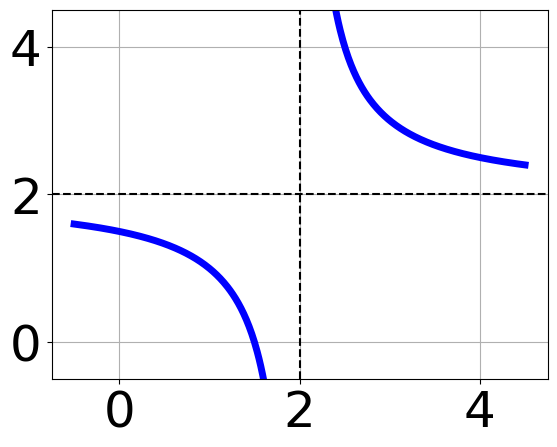
\includegraphics[width=0.5\textwidth]{../Figures/rationalGraphToEquationC.png}
\end{center}


The solution is \( f(x) = \frac{1}{x - 2} + 2 \), which is option A.\begin{enumerate}[label=\Alph*.]
\item \( f(x) = \frac{1}{x - 2} + 2 \)

This is the correct option.
\item \( f(x) = \frac{1}{(x - 2)^2} + 2 \)

Corresponds to thinking the graph was a shifted version of $\frac{1}{x^2}$.
\item \( f(x) = \frac{-1}{x + 2} + 2 \)

Corresponds to using the general form $f(x) = \frac{a}{x+h}+k$ and the opposite leading coefficient.
\item \( f(x) = \frac{-1}{(x + 2)^2} + 2 \)

Corresponds to thinking the graph was a shifted version of $\frac{1}{x^2}$, using the general form $f(x) = \frac{a}{x+h}+k$, and the opposite leading coefficient.
\item \( \text{None of the above} \)

This corresponds to believing the vertex of the graph was not correct.
\end{enumerate}

\textbf{General Comment:} Remember that the general form of a basic rational equation is $ f(x) = \frac{a}{(x-h)^n} + k$, where $a$ is the leading coefficient (and in this case, we assume is either $1$ or $-1$), $n$ is the degree (in this case, either $1$ or $2$), and $(h, k)$ is the intersection of the asymptotes.
}
\litem{
Choose the equation of the function graphed below.

\begin{center}
    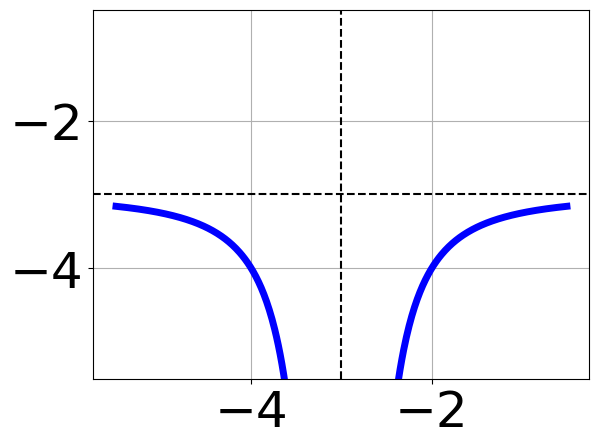
\includegraphics[width=0.5\textwidth]{../Figures/rationalGraphToEquationCopyC.png}
\end{center}


The solution is \( f(x) = \frac{-1}{(x + 3)^2} - 3 \), which is option D.\begin{enumerate}[label=\Alph*.]
\item \( f(x) = \frac{-1}{x + 3} - 3 \)

Corresponds to thinking the graph was a shifted version of $\frac{1}{x}$.
\item \( f(x) = \frac{1}{(x - 3)^2} - 3 \)

Corresponds to using the general form $f(x) = \frac{a}{(x+h)^2}+k$ and the opposite leading coefficient.
\item \( f(x) = \frac{1}{x - 3} - 3 \)

Corresponds to thinking the graph was a shifted version of $\frac{1}{x}$, using the general form $f(x) = \frac{a}{(x+h)^2}+k$, and the opposite leading coefficient.
\item \( f(x) = \frac{-1}{(x + 3)^2} - 3 \)

This is the correct option.
\item \( \text{None of the above} \)

This corresponds to believing the vertex of the graph was not correct.
\end{enumerate}

\textbf{General Comment:} Remember that the general form of a basic rational equation is $ f(x) = \frac{a}{(x-h)^n} + k$, where $a$ is the leading coefficient (and in this case, we assume is either $1$ or $-1$), $n$ is the degree (in this case, either $1$ or $2$), and $(h, k)$ is the intersection of the asymptotes.
}
\litem{
Choose the graph of the equation below.
\[ f(x) = \frac{1}{(x + 1)^2} - 2 \]The solution is the graph below, which is option E.
    \begin{center}
        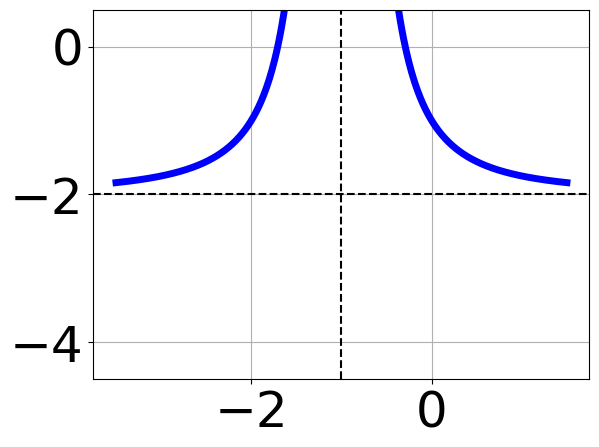
\includegraphics[width=0.3\textwidth]{../Figures/rationalEquationToGraphCopyEC.png}
    \end{center}\begin{enumerate}[label=\Alph*.]
\begin{multicols}{2}
\item 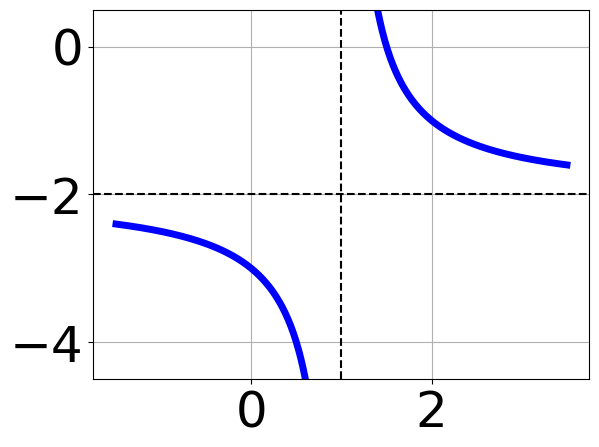
\includegraphics[width = 0.3\textwidth]{../Figures/rationalEquationToGraphCopyAC.png}
\item 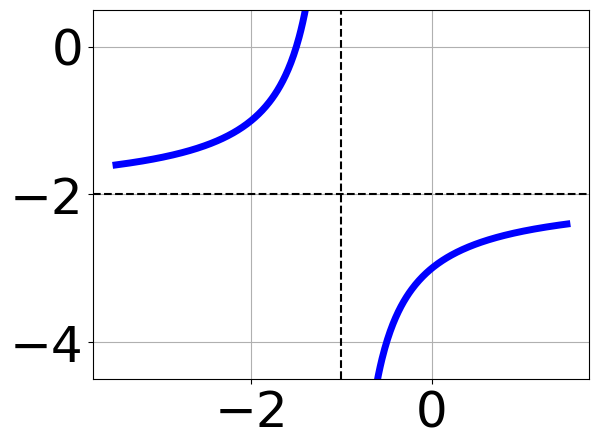
\includegraphics[width = 0.3\textwidth]{../Figures/rationalEquationToGraphCopyBC.png}
\item 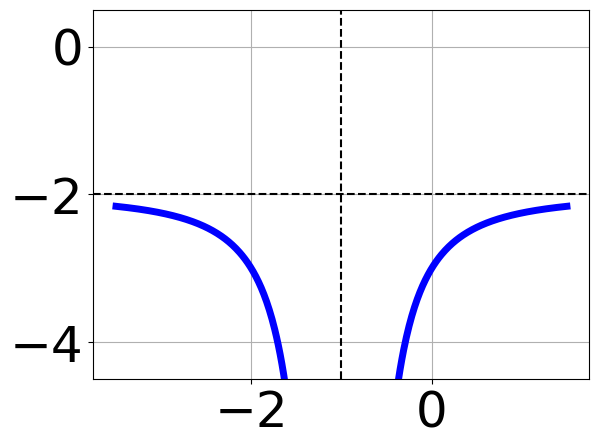
\includegraphics[width = 0.3\textwidth]{../Figures/rationalEquationToGraphCopyCC.png}
\item 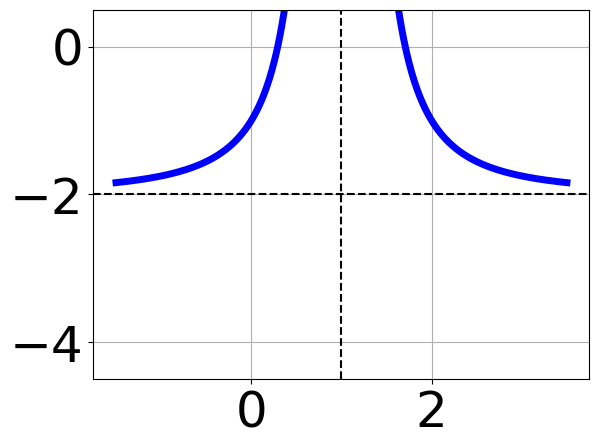
\includegraphics[width = 0.3\textwidth]{../Figures/rationalEquationToGraphCopyDC.png}
\end{multicols}\item None of the above.\end{enumerate}
\textbf{General Comment:} Remember that the general form of a basic rational equation is $ f(x) = \frac{a}{(x-h)^n} + k$, where $a$ is the leading coefficient (and in this case, we assume is either $1$ or $-1$), $n$ is the degree (in this case, either $1$ or $2$), and $(h, k)$ is the intersection of the asymptotes.
}
\litem{
Solve the rational equation below. Then, choose the interval(s) that the solution(s) belongs to.
\[ \frac{-2x}{3x -2} + \frac{-6x^{2}}{6x^{2} +11 x -10} = \frac{-4}{2x + 5} \]The solution is \( \text{All solutions are invalid or lead to complex values in the equation.} \), which is option A.\begin{enumerate}[label=\Alph*.]
\item \( \text{All solutions lead to invalid or complex values in the equation.} \)

* The equation leads to solving $2x^{2} +2 x -8=0$, which leads to complex solutions. This is the correct option.
\item \( x \in [0.65,0.68] \)

$x = 0.667$, which corresponds to solving $3x -2 = 0$ and treating it as a solution to the equation.
\item \( x \in [-2.54,-2.47] \)

$x = -2.500$, which corresponds to solving $2x + 5 = 0$ and treating it as a solution to the equation.
\item \( x_1 \in [-2.6, -2.56] \text{ and } x_2 \in [1.56,2.56] \)

$x = -2.562 \text{ and } x = 1.562$, which corresponds to making the discriminant from the Quadratic Formula positive to avoid complex solutions.
\item \( x_1 \in [0.65, 0.68] \text{ and } x_2 \in [-3.5,-1.5] \)

$x = 0.667 \text{ and } x = -2.500$, which corresponds to solving $3x -2 = 0$ and $2x + 5 = 0$ and treating them as solutions to the equation.
\end{enumerate}

\textbf{General Comment:} Distractors are different based on the number of solutions. Remember that after solving, we need to make sure our solution does not make the original equation divide by zero!
}
\litem{
Solve the rational equation below. Then, choose the interval(s) that the solution(s) belongs to.
\[ \frac{-3x}{7x + 6} + \frac{-2x^{2}}{-28x^{2} -10 x + 12} = \frac{5}{-4x + 2} \]The solution is \( \text{There are two solutions: } x = -0.634 \text{ and } x = 4.734 \), which is option A.\begin{enumerate}[label=\Alph*.]
\item \( x_1 \in [-0.99, -0.27] \text{ and } x_2 \in [2.73,11.73] \)

* $x = -0.634 \text{ and } x = 4.734$, which is the correct option.
\item \( \text{All solutions lead to invalid or complex values in the equation.} \)


\item \( x \in [0.36,0.75] \)


\item \( x \in [4.07,5.47] \)


\item \( x_1 \in [-0.99, -0.27] \text{ and } x_2 \in [-2.86,2.14] \)


\end{enumerate}

\textbf{General Comment:} Distractors are different based on the number of solutions. Remember that after solving, we need to make sure our solution does not make the original equation divide by zero!
}
\litem{
Determine the domain of the function below.
\[ f(x) = \frac{6}{18x^{2} -6 x -24} \]The solution is \( \text{All Real numbers except } x = -1.000 \text{ and } x = 1.333. \), which is option E.\begin{enumerate}[label=\Alph*.]
\item \( \text{All Real numbers except } x = a, \text{ where } a \in [-3, 1] \)

All Real numbers except $x = -1.000$, which corresponds to removing only 1 value from the denominator.
\item \( \text{All Real numbers except } x = a \text{ and } x = b, \text{ where } a \in [-36, -35] \text{ and } b \in [12, 13] \)

All Real numbers except $x = -36.000$ and $x = 12.000$, which corresponds to not factoring the denominator correctly.
\item \( \text{All Real numbers.} \)

This corresponds to thinking the denominator has complex roots or that rational functions have a domain of all Real numbers.
\item \( \text{All Real numbers except } x = a, \text{ where } a \in [-36, -35] \)

All Real numbers except $x = -36.000$, which corresponds to removing a distractor value from the denominator.
\item \( \text{All Real numbers except } x = a \text{ and } x = b, \text{ where } a \in [-3, 1] \text{ and } b \in [0.33, 6.33] \)

All Real numbers except $x = -1.000$ and $x = 1.333$, which is the correct option.
\end{enumerate}

\textbf{General Comment:} Recall that dividing by zero is not a real number. Therefore the domain is all real numbers \textbf{except} those that make the denominator 0.
}
\litem{
Determine the domain of the function below.
\[ f(x) = \frac{3}{16x^{2} +8 x -24} \]The solution is \( \text{All Real numbers except } x = -1.500 \text{ and } x = 1.000. \), which is option B.\begin{enumerate}[label=\Alph*.]
\item \( \text{All Real numbers except } x = a \text{ and } x = b, \text{ where } a \in [-25.9, -22.9] \text{ and } b \in [14.9, 16.3] \)

All Real numbers except $x = -24.000$ and $x = 16.000$, which corresponds to not factoring the denominator correctly.
\item \( \text{All Real numbers except } x = a \text{ and } x = b, \text{ where } a \in [-2.5, -0.7] \text{ and } b \in [-0.5, 1.4] \)

All Real numbers except $x = -1.500$ and $x = 1.000$, which is the correct option.
\item \( \text{All Real numbers except } x = a, \text{ where } a \in [-2.5, -0.7] \)

All Real numbers except $x = -1.500$, which corresponds to removing only 1 value from the denominator.
\item \( \text{All Real numbers except } x = a, \text{ where } a \in [-25.9, -22.9] \)

All Real numbers except $x = -24.000$, which corresponds to removing a distractor value from the denominator.
\item \( \text{All Real numbers.} \)

This corresponds to thinking the denominator has complex roots or that rational functions have a domain of all Real numbers.
\end{enumerate}

\textbf{General Comment:} Recall that dividing by zero is not a real number. Therefore the domain is all real numbers \textbf{except} those that make the denominator 0.
}
\litem{
Choose the graph of the equation below.
\[ f(x) = \frac{-1}{x - 3} - 3 \]The solution is the graph below, which is option A.
    \begin{center}
        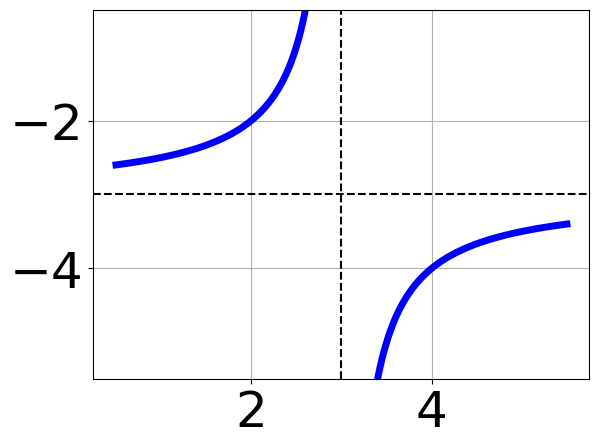
\includegraphics[width=0.3\textwidth]{../Figures/rationalEquationToGraphAC.png}
    \end{center}\begin{enumerate}[label=\Alph*.]
\begin{multicols}{2}
\item 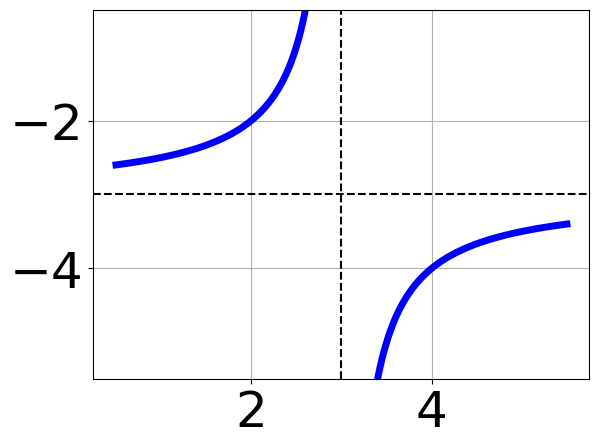
\includegraphics[width = 0.3\textwidth]{../Figures/rationalEquationToGraphAC.png}
\item 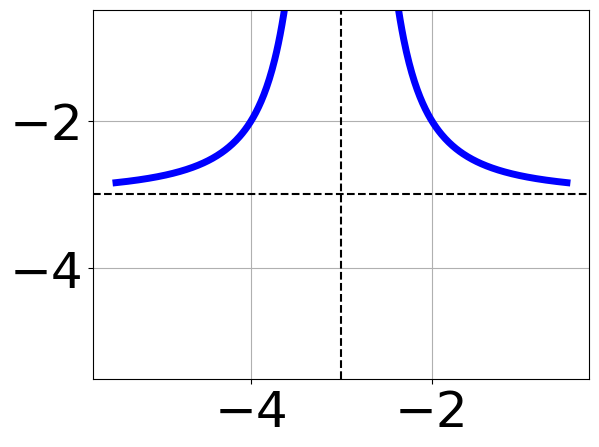
\includegraphics[width = 0.3\textwidth]{../Figures/rationalEquationToGraphBC.png}
\item 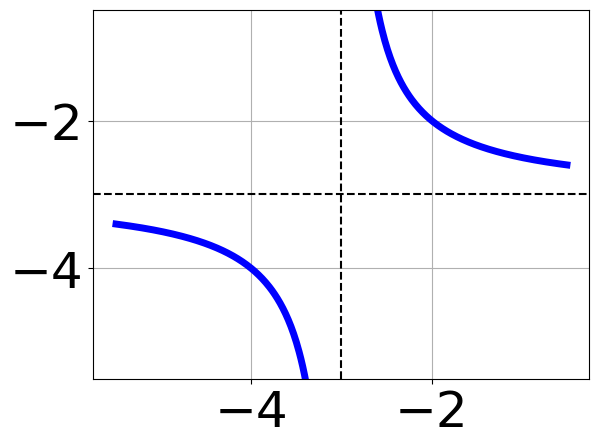
\includegraphics[width = 0.3\textwidth]{../Figures/rationalEquationToGraphCC.png}
\item 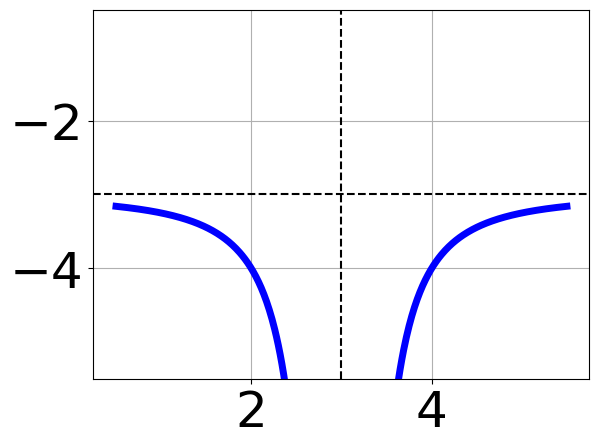
\includegraphics[width = 0.3\textwidth]{../Figures/rationalEquationToGraphDC.png}
\end{multicols}\item None of the above.\end{enumerate}
\textbf{General Comment:} Remember that the general form of a basic rational equation is $ f(x) = \frac{a}{(x-h)^n} + k$, where $a$ is the leading coefficient (and in this case, we assume is either $1$ or $-1$), $n$ is the degree (in this case, either $1$ or $2$), and $(h, k)$ is the intersection of the asymptotes.
}
\litem{
Solve the rational equation below. Then, choose the interval(s) that the solution(s) belongs to.
\[ \frac{88}{88x + 55} + 1 = \frac{88}{88x + 55} \]The solution is \( \text{all solutions are invalid or lead to complex values in the equation.} \), which is option A.\begin{enumerate}[label=\Alph*.]
\item \( \text{All solutions lead to invalid or complex values in the equation.} \)

*$x = -0.625$ leads to dividing by 0 in the original equation and thus is not a valid solution, which is the correct option.
\item \( x \in [-0.62,0.38] \)

$x = -0.625$, which corresponds to not checking if this value leads to dividing by 0 in the original equation and thus is not a valid solution.
\item \( x_1 \in [-1.62, 0.38] \text{ and } x_2 \in [-1.62,0.38] \)

$x = -0.625 \text{ and } x = -0.625$, which corresponds to getting the correct solution and believing there should be a second solution to the equation.
\item \( x_1 \in [-1.62, 0.38] \text{ and } x_2 \in [0.62,1.62] \)

$x = -0.625 \text{ and } x = 0.625$, which corresponds to getting the correct solution and believing there should be a second solution to the equation.
\item \( x \in [-0.38,2.62] \)

$x = 0.625$, which corresponds to not distributing the factor $88x + 55$ correctly when trying to eliminate the fraction.
\end{enumerate}

\textbf{General Comment:} Distractors are different based on the number of solutions. Remember that after solving, we need to make sure our solution does not make the original equation divide by zero!
}
\end{enumerate}

\end{document}